\begin{figure}[t]
  \center
  \begin{framed}\centering
  \def\layersep{4cm}
  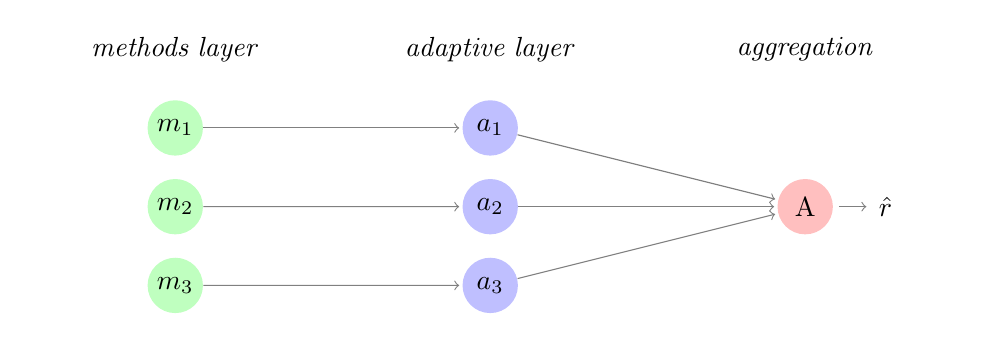
\begin{tikzpicture}[shorten >=1pt,->,draw=black!50, node distance=\layersep]

    \tikzstyle{every pin edge}=[<-,shorten <=2pt]
    \tikzstyle{neuron}=[circle,fill=black!25,minimum size=20pt,inner sep=0pt]
    \tikzstyle{input neuron}=[neuron, fill=green!25];
    \tikzstyle{output neuron}=[neuron, fill=red!25];
    \tikzstyle{hidden neuron}=[neuron, fill=blue!25];
    \tikzstyle{annot} = [text width=10em, text centered]

    % Draw the input layer nodes
    \foreach \name / \y in {1,...,3}
    % This is the same as writing \foreach \name / \y in {1/1,2/2,3/3,4/4}
        \node[input neuron] (I-\name) at (0,-\y) {$m_{\y}$};

    % Draw the hidden layer nodes
    \foreach \name / \y in {1,...,3}
        \node[hidden neuron] (H-\name) at (\layersep,-\y cm) {$a_{\y}$};

    % Draw the output layer node
    \node[output neuron,pin={[pin edge={->}]right:$\hat{r}$}, right of=H-2] (O) {A};

    % Connect every node in the input layer with every node in the
    % hidden layer.
    \foreach \source in {1,...,3}
         \path (I-\source) edge (H-\source);

    % Connect every node in the hidden layer with the output layer
    \foreach \source in {1,...,3}
        \path (H-\source) edge (O);

    % Annotate the layers
    \node[annot,above of=H-1, node distance=1cm] (hl) {\emph{adaptive layer}};
    \node[annot,left of=hl] {\emph{methods layer}};
    \node[annot,right of=hl] {\emph{aggregation}};
  \end{tikzpicture}

  \vspace{1em}
  \caption[Stacked User Modeling]{
    Stacked user modeling:
    The method layer consists of three ordinary modeling methods,
    each predicting the rating between a user and an item.
    The adaptive layer estimates how well each modeling method
    will perform for the current user and item,
    and weighs the predictions accordingly.
    The aggregation layer combines these weighted combinations 
    into one final score.
  }
  \label{fig:stackedusermodeling}
\end{framed}\end{figure}
